\documentclass[10pt,a4paper,twoside,openright]{book}
\usepackage{dei}
%\usepackage[all]{xy}
%\usepackage{supertabular}

\usepackage{url}
\usepackage[pdftex,
	pdftitle					= {creating urban scenery using multimodal interfaces},
	pdfauthor					= {Jos� Pedro Dias},
	bookmarks         = true,				% do bookmarks
	bookmarksnumbered = true,				% keep sedtion numbers
%	pdfpagemode       = None,				% start with closed bookmarks
	pdfstartview      = FitH,				% starting view scale
%	pdfpagelayout     = SinglePage,	% one page at a time
	linkcolor					= black,			% links inside the document
	citecolor					= black,			% for cites
%	linkcolor					= blue,				% links inside the document
%	citecolor					= red,				% for cites
%	urlcolor					= green,			% for urls
	colorlinks        = true]{hyperref}


%\def\hellow{
%	\textcolor{red}{HELLO!}
%}
%
%% with receiving param
%\def\hellow2#1{
%	\textcolor{red}{begin #1 end}
%}
%
%% alternative way of starting ending a command
%\def\hellow3#1{
%	{\bf#1}
%	\begin{bf}#1\end{bf}
%}

% show TODOs
\def\TODO#1{
	%\glossary{#1}
	\textcolor{red}{\textbf{TODO:} #1}
}

% hide TODOs
%\def\TODO#1{}



\begin{document}

%capa
\thispagestyle{empty}%

\includegraphics[width=9cm]{logo-ist}
\vspace{4.5cm}
\begin{center}
\Large{\textbf{{\fontfamily{phv}\selectfont Creating Urban Scenery}}}\\
\Large{\textbf{{\fontfamily{phv}\selectfont Using Multimodal Interfaces}}}\\
\vspace{1.5cm}
\large{\textbf{{\fontfamily{phv}\selectfont Jos� Pedro do Sacramento Aleixo Dias}}}\\
\vspace{1.5cm}
\large{{\fontfamily{phv}\selectfont Disserta��o para obten��o do Grau de Mestre em}}\\
\Large{\textbf{{\fontfamily{phv}\selectfont Engenharia Inform�tica e de Computadores}}}\\
\vspace{1.5cm}
\large{\textbf{{\fontfamily{phv}\selectfont J�ri}}}\\
\end{center}
\normalsize{{\fontfamily{phv}\selectfont Presidente: Prof. Xxxxx Xxxxx Xxxxxx Xxx Xxxxxx xx Xxxxx}}\\
\normalsize{{\fontfamily{phv}\selectfont Orientador: Prof. Xxxxxx Xxxxx Xxxxxx Xxxx xx Xxxxx}}\\
\normalsize{{\fontfamily{phv}\selectfont Vogais: Prof. Xxxxxx Xxxxxx Xxxxxxx xx Xxxxx}}\\
\vspace{1cm}
\begin{center}
\large{\textbf{{\fontfamily{phv}\selectfont Setembro de 2007}}}\\
\end{center}

\newpage

\frontmatter

\chapter*{Resumo}
\addcontentsline{toc}{chapter}{Resumo}
\chapter*{Resumo}
\addcontentsline{toc}{chapter}{Resumo}

%\TODO{CHECK FOR MAXIMUM 250 WORDS!}

Desenvolveu-se um sistema para ecr�s de larga escala,
fazendo uso de ponteiros laser convencionais como interface de entrada.
Este sistema suporta uso colaborativo.
Foi criada uma interface inovadora de modo a suportar a interac��o com tais dispositivos,
baseada no conceito de port�es e menus circulares n�o-intrusivos.



% implementation / features


Os utilizadores s�o capacitados de navegar num mundo virtual utilizando um conjunto de
modos de navega��o, nomeadamente: primeira pessoa, modo b�ssola e modo examinar, assim como
um modo de v�o multimodal, integrando comandos de voz e movimento dos bra�os.
Podem ser criadas e modeladas formas simples, fazendo uso de um conjunto de ferramentas
de modela��o que definem um novo modelo de interac��o para a modela��o de objectos.
Podem ser instanciados edif�cios a partir de um conjunto de estilos de fachada pr�-existentes,
pelo desenho da sua planta e al�ado, dando origem a edif�cios �nicos.
Estilos adicionais podem ser gerados, recorrendo a um formato XML para definir regras de distribui��o de elementos nas fachadas de edif�cios.
Os edif�cios e restantes objectos podem ser transformados e clonados.
Podem anexar-se anota��es a objectos, de modo a suportar cen�rios de revis�o.
Um processo alternativo de cria��o de edif�cios � proposto para tirar proveito
do sistema tanto nas primeiras fases como na apresenta��o de projectos.

A arquitectura do sistema � descrita, seguida de detalhes de implementa��o e testes de avalia��o.
� demonstrado que os utilizadores conseguiram fazer uso das capacidades do sistema com sucesso.
As conclus�es do projecto e trabalho futuro fecham este documento.


%\TODO{CHECK FOR 4 -- 6 KEYWORDS!}
\textbf{Palavras-Chave:}
tra�o,
edif�cio,
interface multimodal,
navega��o,
ecr� larga escala,
BREP


\chapter*{Abstract}
\addcontentsline{toc}{chapter}{Abstract}
\chapter*{Abstract}
\addcontentsline{toc}{chapter}{Abstract}

\TODO{review and summarize this part, add implementation part.}

% context and problem
Nowadays the architectural project workflow is highly segmented
between the creative part and the CAD modeling part.
It starts with the architects drafting hand-made sketches of building designs
to study viable designs and validating them with clients, a stage without computer usage, 
with all participants on location using pen and paper.
Later on a set of documents is generated from the ground up on CAD software, 
using desktop computers and WIMP interfaces.

% motivation, goals
There's an increasing availability of alternative methods for both sketching, navigation and visualization
of 3D scenes which can enrich the design process and provide a better experience for both
building drafting, visualization and review.
We're committed to developing a multimodal distributed system to fulfill these goals
using tablet PCs or other devices facing a powerwall.
%We're committed to developing a multimodal system allowing multi-user scene navigation,
%building draft building designs, navigation and content reviewing.
It is thought out to integrate the architectural workflow as a creative and reviewing tool
to complement the early stages of architectural design.

% document organization
This survey begins with an analysis of projects with similar goals,
followed by a set of issues to handle:
how to get input from users,
display interactive content to them,
make shape creation and transformation possible and
allow scene navigation
%provide content reviewing capabilities.
A comparative analysis between architecture creation systems available in the market is then conducted and
finally conclusions are reached and directions for project execution defined.

\textbf{Keywords:} urban architecture, city, building, multimodal interaction, navigation, content reviewing


\chapter*{Acknowledgements}
\addcontentsline{toc}{chapter}{Acknowledgements}
\chapter*{Acknowledgements}
\addcontentsline{toc}{chapter}{Acknowledgements}

The author would like to thank his supervisor Prof. Joaquim Jorge
for his guidance.

He would like to thank his coleagues Bruno Ara�jo, Ricardo Jota and Lu�s Bruno
the support a team work during the ImmiView period.

He would like to thank Jos� Ant�nio Gon�alves for taking part it the
motion tracking navigation mode and all the test users who volunteered both
in Glasgow and in Lisbon.

% and Tiago Guerreiro for his experience
%and enthusiastic role as an investigator.

He would like most of all to thank his wife, family and friends for all the love and support.

%This has been a long road and a very fulfilling one. I hope my work is appreciated.

\newpage
\renewcommand\contentsname{Table of Contents}
\tableofcontents\newpage
\listoffigures
\addcontentsline{toc}{chapter}{\listfigurename}\newpage
\listoftables
\addcontentsline{toc}{chapter}{\listtablename}\newpage
\chapter*{List of Acronyms}
\addcontentsline{toc}{chapter}{List of Acronyms}
\chapter*{List of Acronyms}
\addcontentsline{toc}{chapter}{List of Acronyms}

\TODO{review these}

\begin{tabular}{ll}

\textbf{AICI} & Open Scene Graph -- asdasd asd \\

\textbf{OpenSG} & Open Scene Graph -- asdasd asd \\

\textbf{OSGA} & Window Icon Menu Pointing device -- asdasd asd \\

\textbf{WIMP} & Window Icon Menu Pointing device -- asdasd asd \\

\textbf{XML} & Window Icon Menu Pointing device -- asdasd asd \\

\end{tabular}


%\part{Report}
\mainmatter

\begintodo

\chapter{Introduction}
% Context + Problem

% http://en.wikipedia.org/wiki/Architecture

\subsection{The Evolution of Architecture}
Architecture is the art and science of designing buildings and structures.
It is an interdisciplinary field which has similarities to applied science and
engineering, but unlike them, focusing on functional and feasibility aspects of design, 
architecture deals with building costs, space and volume, materials and lighting
in order to achieve an aesthetically pleasing result.

For centuries methods and norms have arisen. Architects tools of work were based on paper and ruler.
With the evolution of computational power throughout the last century, 
increasingly more complete, fast and robust Computer Aided Design (CAD) systems were developed and so did
devices capable of manipulating architectural entities -- such as the mouse, trackball, tablet, etc.

\subsection{Current Workflow for Building Design}
% only geographical, drawings?
Elaborating architectural designs usually starts by drawing rough sketches of the subject
in order to convey form, proportion and lighting.
Relevant geographical data about the location where the building is to be established is acquired.
A series of two dimensional drawings is created in order to precisely define building features, dimensions and location.
These drawings serve as input for civil engineers and the rest of staff responsible for constructing the building.
Three dimensional drawings and brochures are created and scale models are built,
allowing people with no architectural background to better perceive the building before it is built.

Nowadays architecture is slowly but steadily embracing usage of computers in the designing process.
Authoring systems such as Autodesk's AutoCAD
\cite{SITE-AUTOCAD}
are currently used to produce a set of views and floor plans necessary to construct a building.
These systems are optimized for such tasks, having limited support for general 3D volume and surface creation
and rely heavily in desktop interfaces with keyboard/mouse.

The creation of 3D drawings and brochures for marketing purposes is common practice.
It relies in techniques such as
ray tracing \cite{SITE-POVRAY},
radiosity,
physically accurate light simulation \cite{SITE-MAXWELL}, \cite{SITE-INDIGO}; 
High Dynamic Range Imaging (HDRI), etc.
These techniques produce believable results but take too much time to render in real time.

% articles for bsps, octtrees, light rendering alg?
Another application for data coming from CAD systems is the generation of worlds optimized for navigation.
Performance is paramount in these systems so algorithms such space partition --
Binary Space Partitions (BSPs) for closed space rendering,
OctTrees for open space rendering --
and multiple Levels Of Detail (LOD) for each shape are commonly used.
The compromise between believability and fast rendering times is assured with techniques such as
light maps and using recent graphics card's Graphics Processing Unit (GPU),
shifting complex computer graphics algorithms out of the Central Processing Unit (CPU),
obtaining frame rates otherwise impossible with current hardware.

There are numerous 3D engines capable of presenting such worlds with good performance.
The major drawbacks in their usage rely on how the user navigates the scene --
most systems use the popular interface featured in most first or third person shooters,
relying on mouse/keyboard for input --
and on the lack of support for out-of-the-box interaction with shapes.
\TODO{UGLY PHRASE!}

\newpage
Exporting the geometry from a CAD program, which is a common solution, comes with several problems,
as stated by Alberto Raposo et al.\cite{CADVR06}:
\begin{description}
	\item[Low performance] -- due to unneeded model complexity;
	\item[Lack of realism] -- usually users of CAD programs don't associate material
	or texture data to objects;
	\item[Inadequate treatment of geometry] -- the conversion often occurs with loss of
	geometry, precision and errors such as badly oriented normals.
\end{description}

\subsection{Benefits and Goals of an Integrated Approach}
% client side benefits
Using a computer system to present a virtual building with the purpose of selling an idea,
doing real estate business or simulating virtual tours demands better metaphors,
better interface design and the least possible cluttering of the view in order
to achieve a richer user experience and get an overall good impression.
Navigating and reviewing content should be simple tasks to perform.

% architect benefits
From the architect's point of view, using such a system early in the process,
if preceded by geographical data capturing,
allows him to better perceive the construction area, which improves a seamless building integration.
Additionally, applying such a system in the building design workflow allows the generation
of models able to complement or even replace the first prototyping stages,
commonly represented nowadays by rough sketches.
The possibility of collaborative remote design and content reviewing offers a cheaper
alternative for distributed projects and allows a shorter validation cycle with the clients.

\subsection{Document Structure}
% structure for the rest of the document
This document continues with the identification of various problems that need to be solved in order
to fulfill these goals.
A series of projects in this area is then discussed.
Several subjects are then analyzed:
input modalities (using laser pointers, tablet PC pen, motion tracking and voice commands);
output modalities (using tablet PCs, powerwalls or head mounted displays);
shape creation and transformation (for modeling simple buildings, their translation, scaling, etc.);
scene navigation (using several modalities) and
content reviewing (by creating and editing shape attached annotations).
Later on a comparative analysis between applications in the market allowing architecture modeling is conducted.
The document ends with a set of conclusions and directions for future work in
addressing this subject.


\chapter{Related Work}
\chapter{Related Work}

\TODO{intro to related work}

\section{Existing Solutions}

% EXISTING SOLUTIONS
% existing solutions

% intro

Three systems will be discussed in this area, each one 
withstanding common goals with the idealized solution.

ARVIKA is the biggest project so far in the
Augmented Reality domain. It offers a working solution to aid in industrial tasks but leaves most
of the regular user interfaces intact, leaving space for improvements at this level.
Additionally, it lacks an authoring tool to provide end-users means to set up scenarios in a friendlier manner.

Speech and Gestures shows a project where the Google Earth \cite{SITE-EARTH} application
-- a single user system that allows navigation in a world representation -- has been adapted to
work on a multi-touch surface with speech recognition.
The adapting work provided feedback about the limitations such software faces 
and offers a working solution to map most Google Earth actions to speech and gesture commands.

Finally, Digital Whiteboard provides a solution for multi-user digital
whiteboards where each user handles a palmtop serving as both the user's palette and
private composing area, supporting text and drawings input.
A technique called pick-and-drop is then explained. It is used to allow a user to transfer
the contents of the palmtop on the shared whiteboard.

\TODOL{SEE NEWEST ARTICLE REPOSITORY, NAMELY instant architecture and IPCity}


\subsection{ARVIKA, 2003}

ARVIKA \cite{ARVIKA} is a project with sponsoring from the
German Federal Ministry of Education and Research that was implemented between 1999 and 2003.
It focused on the development of Augmented Reality (AR) technologies to aid in performing industrial tasks.
The consortium involved several industrial partners such as Volkswagen, BMW, Siemens and Airbus.

\begin{figure}[!ht]
    \centering
    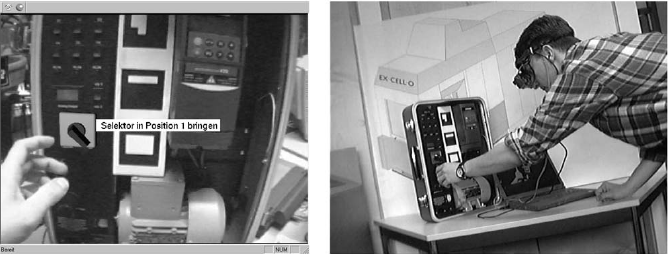
\includegraphics[width=10cm]{gfx/arvika.png}
    \caption{The augmented view seen from the HMD; a user of the ARVIKA system}
    \label{FIG-ARVIKA}
\end{figure}

An expert in the industrial area would carry a head-mounted display (HMD) with a camera mounted on it.
The real-time captured video was then interpreted and markers extracted from the image.
The camera's positioning and orientation were estimated and the HMD view was enriched with virtual objects
(see figure \ref{FIG-ARVIKA}, left).
The framework was distributed in the form of an ActiveX plug-in for the Internet Explorer browser
named ARBrowser.

% discussion

Weidenhausen et al. \cite{ARVIKA-LESSONS} consider the deployment of the project as an ActiveX component
to be an advantage since it is based on a widespread program (Internet Explorer) and allowed developers
to create task scenarios with familiar technologies such as JavaScript and HTML.
Although the world's largest research project in the area, ARVIKA focused too much on the technical problems
regarding AR and little effort was spent on the creation of a suitable user interface.
The authors agree on a point: ``most people judge the usefulness of a technology mainly by its user interface''.
Therefore this particular topic became work for future project iterations.
ARVIKA was meant to support many industrial scenarios -- development, production and services for several
industrial partners on different domains.
Creating a scenario was a time consuming task -- taking several days, according to Weidenhausen et al.
-- and required extensive knowledge in 3D modeling tools and VRML. No authoring capabilities were given to end-users.
This problem was identified as paramount and an authoring tool was scheduled for future development,
supporting generic task creation with parameters controlled by the users.



\subsection{Speech and Gestures on a Multi-User Tabletop, 2006}

Tse et al. \cite{SP-GEST-TTOP} developed a multimodal interface on top of Google Earth \cite{SITE-EARTH}
to be run on a multi-touch table.
The system allows multi-user collaboration with touch and voice commands.

The main problems found in adapting Google Earth reside in the fact that it was thought out as a single user program,
where only one action could be done at a time.
In this scenario several users could be disposed around the table with different orientations,
so text readability problems arose.
Additionally, user interface components such as the compass were placed at fixed points on the screen,
an approach that does not favor multi-user scenarios.
At 1024 x 768 resolution it was estimated that 42\% of the screen was originally consumed by GUI elements.
Since all users shared the surface, turn-taking had to be agreed by the users,
not being enforced by the system (see figure \ref{FIG-SP-TABLETOP}).
Most Google Earth interactive actions were mapped into gestures,
leaving the most abstract actions for voice commands activation (see figure \ref{FIG-SP-TABLETOP2}).


\begin{figure}[!ht]
    \centering
    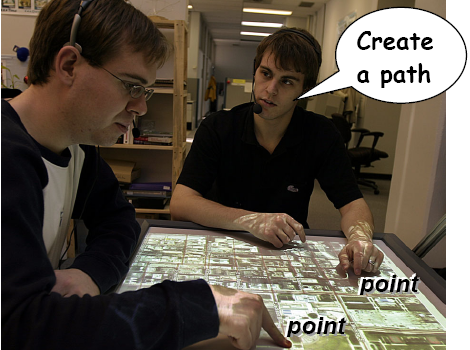
\includegraphics[width=7cm]{gfx/sp-gest-ttop.png}
    \caption{Two users collaborating on a Google Earth tabletop session}
    \label{FIG-SP-TABLETOP}
\end{figure}

\begin{figure}[!ht]
    \centering
    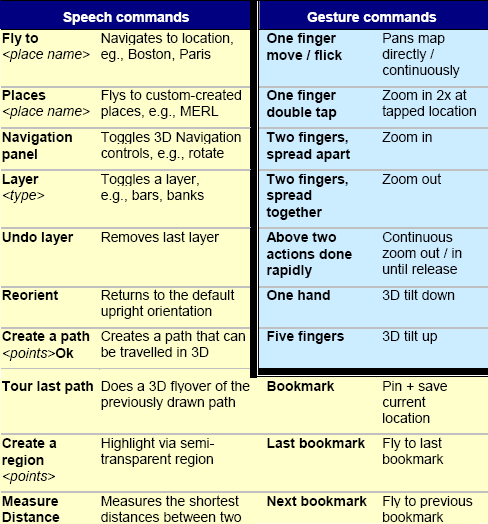
\includegraphics[width=8cm]{gfx/sp-gest-ttop2.png}
    \caption{The suggested speech and gesture interface for Google Earth}
    \label{FIG-SP-TABLETOP2}
\end{figure}

%\paragraph{Discussion}

This project shows the difficulties in adapting a production software thought out
for single user WIMP\footnote{Window Icon Menu Pointing device} interfaces for the support of collaborative scenarios.
A multimodal interface was built over the existing one, mapping most of its commands.
The set of obtained commands is a good example of how navigation can be performed on
3D scenery using a multimodal interface.
Google Earth is a good example of a navigation system suited for single user interaction.
It provides several functionality and could support the creation of buildings.
Making use of its large dataset of satellite images and topography would be excellent
for the target system.


\subsection{Digital Whiteboard, 1998}

Rekimoto \cite{WBOARD} presents a digital whiteboard where each participant is given
a palmtop computer to handle. It works as a tool palette, remote commander, text entry box as
well as a temporary data buffer during whiteboard collaboration interaction.

\begin{figure}[!ht]
	\centering
	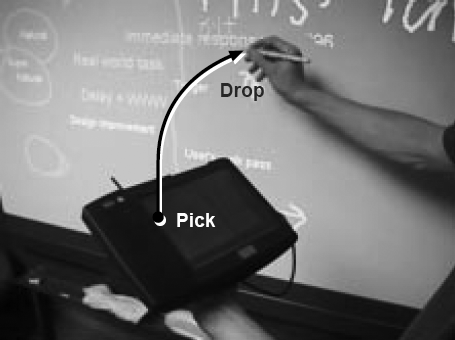
\includegraphics[width=6cm]{gfx/wboard.png}
	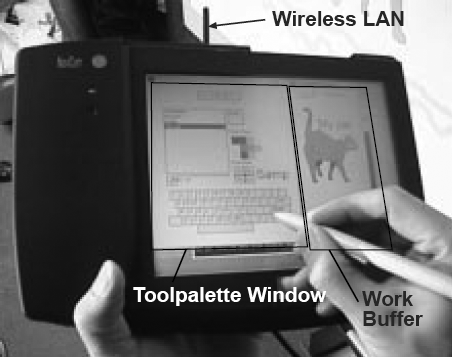
\includegraphics[width=6cm]{gfx/wboard2.png}
	\caption{Digital Whiteboard:
		Pick-and-drop interaction;
		Working areas for each participant's palmtop.}
	\label{FIG-WBOARD}
\end{figure}

The solution involves each participant carrying a pen and a palmtop,
with the pen working on both palmtop and whiteboard.
A direct manipulation method called Pick-and-drop(see Fig. \ref{FIG-WBOARD} left) was developed.
It allows a user to pick an object in his palmtop and dropping it on the whiteboard.
From the implementation point of view data is transferred through the network,
but from the user's perspective this technique allows him to pick up digital data
as if it were a physical object.
Text entry is performed on the palmtop and each user can choose the method he favors
(i.e.: handwritten recognition, soft keyboard, etc) for entering text.
No menus or tool palettes exist on the whiteboard -- they're available on each user's palmtop.
The main window is a multi page tool panel.
A user can flip to several tool palette pages, with the remaining area available as a temporary work buffer.
Users can store data elements in this window and paste them to the whiteboard
using Pick-and-Drop operations. (see Fig. \ref{FIG-WBOARD} right).

Rekimoto concludes that by putting many functions on palmtops,
users tend to concentrate too much on their own palmtop devices,
degrading mutual awareness among the participants.
Pick-and-Drop often worked better than drag-and-drop,
particularly when user had to move objects for a long distance.
Drag-and-drop forces a user to keep the pen tip in contact
with the board during the entire operation,
a restriction not suitable for large display surfaces.

%\paragraph{Discussion}

The solution where each user carries a palmtop for the creation of content such as note taking
is suitable for an architectural design and review scenario.
It grants the user the power to draw, type text or compose graphics 
independently from one another and then replicating the information on the whiteboard.
On the other hand there's the danger of users focusing too much on their paltop and losing
awareness of what's happening at the whiteboard.


\section{Approaches}

The set of available motion tracking techniques for gathering user input is discussed.
The most common setups for rendering virtual reality scenes are compared.
The shape creation projects Sesame and SmartPaper are analysed and three scene navigation concepts are visited.

\subsection{Input Modalities}

\subsubsection{Motion Tracking Systems}


Welch and Foxlin \cite{MT-BULLET} conducted a survey on motion tracking systems,
comparing each solution in terms of cost, precision and capacity to solve the tracking problem.
The main group of purposes for motion tracking applications was identified:
view control, navigation, object selection or manipulation, instrument tracking and avatar animation.
There are motion tracking systems available based on measurements of mechanical, inertial, acoustic, magnetic,
optical and radio frequency sensors, each approach bearing its advantages and limitations.
The most robust solution lies in combining two technologies,
such as a hybrid between inertial and acoustic sensors
-- the former providing 6 degrees of freedom data and the latter reading precise positioning for each artifact.

%\TODOL{BRIDGE WITH STT SYSTEM?, MORE INFO EXTRACTED FROM SOURCE?}

%\paragraph{Discussion}

One can envision the proposed solution to use motion tracking to allow users to change their
point of view in the program, navigate the scene, select and manipulate objects, a subset
of functionality identified by Welch and Foxlin.

\subsubsection{Augmented Reality versus Immersive Virtual Reality}

According to Azuma \cite{OVERVIEW-AR} Augmented Reality should be used
when the collaboration task is co-located,
when there is tangible object interaction and enhanced interaction in the real world.
Immersive Virtual Reality is preferred on scenarios with shared views and
remote collaboration.

%\TODOL{MORE CONTENT FROM THIS ARTICLE?}

%\paragraph{Discussion}
%There haven't been set any goals that force the Augmented Reality approach for such a system.
Sharing views and doing collaboration are two expected features of this system so
Virtual Reality is the choice to make. No Augmented Reality feature is found in this project.


%\TODO{issuing voice commands}
%\subsubsection{Voice Commands}
%
%\cite{SP-GEST-TTOP}

% OUTPUT MODALITIES
% using the tablet PC's display
% using a powerwall
% using HMDs

In order to obtain an immersive experience, there's a number of hardware
setups commonly available:

\begin{description}
	\item[Head-Mounted Display (HMD)] --
	  Head-mounting displays are glass-shaped devices, projecting a pair of stereo
	  transformed images to the user's retinas.
	  They normally feature a gyroscope or similar apparatus to measure head orientation and tilt.
	  There are two kinds of HMDs: in the former the images are projected in small opaque screens;
	  in the latter the projected surface is translucid, allowing blending of real and virtual worlds.
	  Translucid HMDs are best crafted for Augmented Reality (AR).
	  
		Using an HMD has the benefit of sticking to the user's head and detecting head orientation.
		On the other hand each HMD serves one single user and it has limited resolution.
		Additionally, most users report suffering from fatigue after long periods of
		usage \cite{VREDUC}.
		Opaque HMDs have the additional downside of users being unable to see the real world, 
		which can be confusing as noted by \cite{VANDERPOL}.
			
	\item[Cave Automatic Virtual Environment (CAVE)] --
	  A CAVE is an immersive virtual reality environment where projectors are directed to four,
	  five or all the six walls of a room-sized cube.
	  
		It shares the benefit of enclosing the user's viewing area with HMDs.
		Has a better resolution though.
		The downside is the small number of simultaneous users who can experience the CAVE at the same time.
	
	\item[Power Wall] --
	  A power wall is a large surface, usually planar, filled by an image.
	  The whole image projection is responsibility of a cluster of projectors set up in a wall.
	  Each projector renders part of the surface and the border between projections is ideally minimal.
	  Each projector is controlled by an independent computer.
	  
		Its size and resolution depend entirely on the setup, but normally a wall offers high resolution
		(depends on the number of projectors in the grid and each projector's resolution).
		Due to the large surface of the wall, several users may be served as once. Another benefit
		is users freedom of movement due to users not carrying wires \cite{INTTABLE}.
		The downside is users having to face the wall to experience the image entirely.
\end{description}

\begin{figure}[!ht]
	\centering
	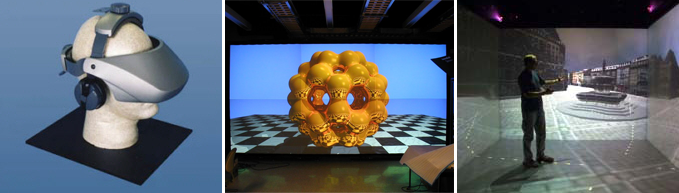
\includegraphics[width=12cm]{gfx/hmd-cluster-cave.png}
	\caption{HMD, Wall, CAVE}
	\label{FIG-HMD-CLUSTER-CAVE}
\end{figure}

Any of these setups is suitable for single user interaction.
In case of a reviewing session, in which at least two participants are required,
CAVE or Wall are better suited, since they alone offer a solution for a small group.

Using a Wall or CAVE presents other challenges: the computers responsible for
generating each projectors' images must be synchronized, its color parameters calibrated
and the viewport must be well cropped.
Several systems exist capable of delivering high performance 3D graphics and
offering the features mentioned above.
Based on scene graphs there are two well established solutions:
OpenSceneGraph\cite{SITE-OSG} and OpenSG\cite{SITE-OPENSG}.


\subsection{Shape Creation}

% SHAPE CREATION AND TRANSFORMATIONS
% for modeling simple buildings
% their translation, scaling, etc.
%\TODO{shape creation}
%\TODO{transformations}

In this section two solutions suitable for conceptual sketching of 3D forms are analyzed.

\subsubsection{SESAME, 2006}

Oh, Stuerzlinger and Danahy \cite{SESAME3D} developed SESAME
(Sketch, Extrude, Sculpt, and Manipulate Easily).
This system tries to provide an interface as powerful and easy to use as 2D sketching on paper.
It is defended by the authors that a 3D model is more easily understood between users
than a regular conceptual design.
It is optimized for modification and allows the creation and editing of volumetric geometry
by extruding 2D contours or sculpting 3D volumes.
It features an enhanced suggestive interface, allowing the creation of lines,
arcs and free-form curves with constraints.
SESAME also supports automatic grouping of objects, i.e., objects related
between themselves (ex: cup on top of table) affect each other.

The user tests conducted comparing SESAME against the popular modeling package
Autodesk 3D Studio Max show that even for experienced 3DSM users
the drawings done with SESAME were more creative and satisfying.

\begin{figure}[!ht]
	\centering
	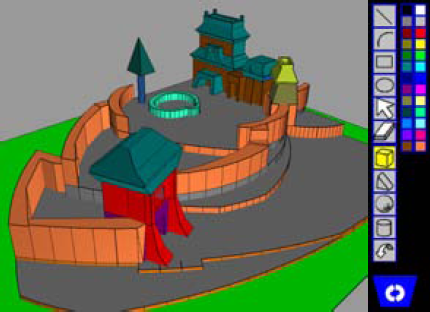
\includegraphics[width=6cm]{gfx/sesame.png}
	\caption{A view of a drawing done in 40 minutes with SESAME}
	\label{FIG-SESAME}
\end{figure}

\paragraph{Discussion}

This is a promising direction for an urban sketching software to go.
The tests against 3D Studio Max were a bit skewed -- the test should
have been conducted against a system of similar approach, such as Google Sketchup.
The offered interface in SESAME appears poorly thought out.

Some constraints may arise from applying these concepts to a multimodal collaborative
system.



\subsubsection{SmartPaper, 2004}

Shesh and Chen \cite{SMARTPAPER} developed SmartPaper, a system designed to support
2D sketching, featuring oversketching capabilities, sketch on 3D, 3D transforms and
CSG operations. It employs a non-photorealistic rendering technique to convey the
drawing a sketchy look.

\begin{figure}[!ht]
	\centering
	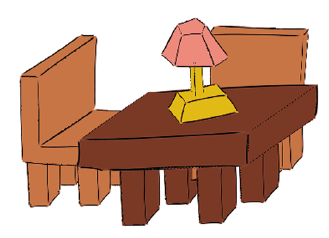
\includegraphics[width=5cm]{gfx/smartpaper.png}
	\caption{Drawing done with SmartPaper}
	\label{FIG-SMARTPAPER}
\end{figure}

\begin{figure}[!ht]
	\centering
	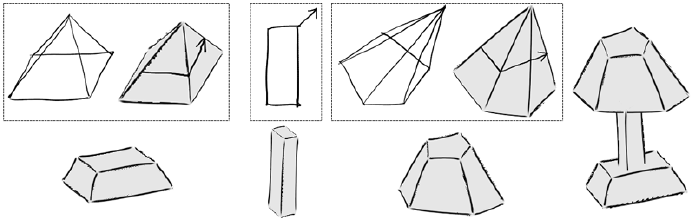
\includegraphics[width=8cm]{gfx/smartpaper2.png}
	\caption{The process of modeling a lamp in SmartPaper}
	\label{FIG-SMARTPAPER2}
\end{figure}

\paragraph{Discussion}

The biggest limitation found in SmartPaper is the lack of curved line support.
Another requirement is that the user must draw all object's edges, not only
the visible ones. In the case of extruded objects this is not problematic, since
the original face would always have to be drawn anyway.
The resulting geometry appears to be irregular but since the goal is to do
conceptual drawings this is not an issue.

\TODOL{RELATE TO OUR PROJECT?}


\subsection{Scene Navigation}


% SCENE NATIGATION

Following is a list of scene navigation solutions.
Each one can contribute to a more powerful and easy interface.


\subsubsection{Smart and Physically Based Camera, 2006}
\label{SMARTCAM-LABEL}

In order to ensure users not ``getting lost'' in the virtual space,
Buchholz, Bohnet and D�llner \cite{SMARTCAM} propose a smart and physically based camera.
Smart in the sense that it is aware of confusing and disorienting viewing situations,
providing means to circumvent them.
Physically based because it is supported by a physics model of 3D motion
to ensure steady, continuous user movements.

Experience shows that people frequently lose track of their location when moving on a 3 dimensional
world.
To solve this problem, the camera must identify situations when to intervene.
For that reason a metric, called orientation value, was created.
Each view is classified by counting its pixels, granting different values:
landmarks get the highest values; terrain gets mid-range values and the sky gets lower values (see Fig. \ref{FIG-SMARTCAM1}, right).
A threshold can then be established and views below the threshold are classified ``disoriented''.
When such an event takes place, smart navigation techniques restrict camera control.
The constraints posed to user control must be as comprehensible as possible.
Camera movement should also be time-coherent and physically sound.

The maintenance strategy solves critical situations such as (see Fig.\ref{FIG-SMARTCAM1}, left):

\begin{enumerate}[a)]
	\item The user rotates the flight direction and causes the camera to look too far beyond the terrain border.
		The rotation is accepted but outweighed by a slight rear movement away from the border.
	\item The user is flying forward beyond the terrain border.
		The maintenance strategy temporarily tilts down the view direction until a maximum angle is reached.
	\item If no more tilting is possible, the strategy rotates the flight direction parallel to the terrain
		to fly along the terrain border.
\end{enumerate}

\begin{figure}[!ht]
	\centering
	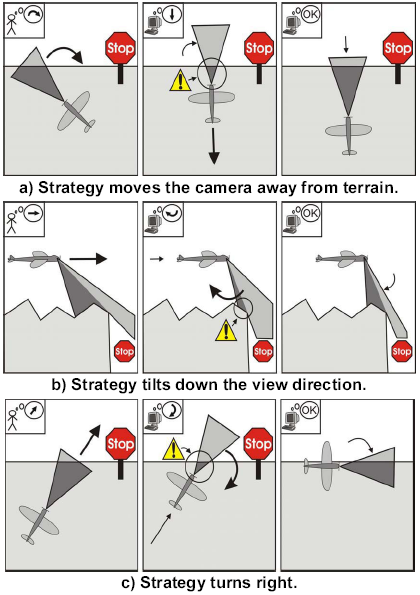
\includegraphics[height=7cm]{gfx/smartcam05-1.png}
	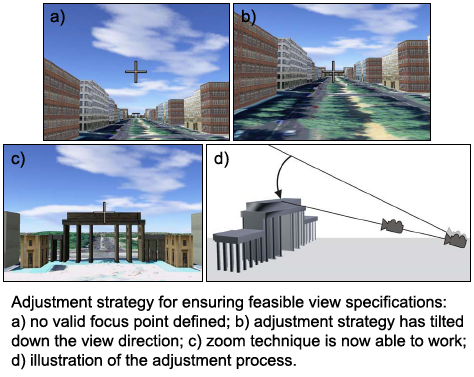
\includegraphics[height=5cm]{gfx/smartcam05-2.png}
	\caption{SPB Cam: Maintenance strategy for keeping high orientation values; Adjustment strategy for ensuring of feasible view specifications.}
	\label{FIG-SMARTCAM1}
\end{figure}

%\paragraph{Discussion}

A camera system such as this can be useful aiding non-experienced users such as clients in navigation tasks
since it maximizes the presence of landmarks in the user's view.
The physically-based engine would grant additional realism to the navigation experience, providing collision
detection, inertia and a spring behavior that would soften camera trajectories.



\subsubsection{Speed-dependent Automatic Zooming, 2000}
\label{SPEEDZOOM-LABEL}

Igarashi and Hinckley \cite{SPEEDZOOM} propose a simple idea for scrolling through large areas of information.
The speed at which the scrolling occurs changes the zooming of the seen area.
This makes sense since the faster the area is scrolling, the longer ahead the user needs to see.

%\paragraph{Discussion}

This could be easily applied to bird's-eye-view maps of large areas.
The scrolling of the map would trigger different zooming factors depending on
the scrolling speed, improving the navigation and exploration of the map.


\subsubsection{Path Drawing for 3D Walkthrough, 1998}
\label{PATH3D-LABEL}

Igarashi et al. \cite{PATH3D} start by identifying the two main types of walkthrough techniques:
\emph{driving}, where the user continuously changes camera position with move and rotation buttons and
\emph{flying}, where the user picks the desired destination with a pointing device and a trajectory is calculated
and animated from the starting position to the picked one.
Each has it disadvantages:
driving requires the user to control the trajectory at all times;
flying lacks expressive power since the user can't control the path neither the final orientation.

The proposed solution is an extension of the flying technique:
the user draws the desired path he wants to take on the screen.
It gets projected onto the walking surfaces and the generated path is animated.
During the animation the user faces the tangential direction related to the path.
This brings the additional advantage of the user being able to define
where he will be facing at the end of the animation.
This technique can be used is two different ways.
The user can draw a long stroke specifying the path at once
or he can draw successions of small strokes (see Fig.\ref{FIG-PATH3D}).

As limitations the authors state the path expressiveness
being limited to the walking surface planes
and the need for the user's avatar to be present on the view
if one wants to draw the path from the user's feet.
 

\begin{figure}[!ht]
	\centering
	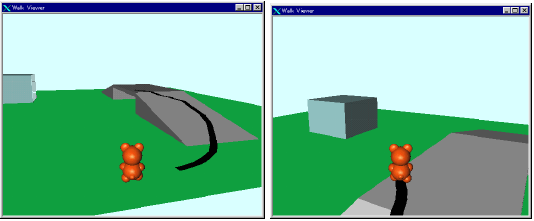
\includegraphics[width=12cm]{gfx/path3d.png}
	\caption{One long path and one short one}
	\label{FIG-PATH3D}
\end{figure}

%\paragraph{Discussion}

This navigation mode could be handy in the review scenario.
Even so this might be hard to apply to the project due to LSD interface limitations.


\TODO{summary of related work}


\chapter{Analysis}
\chapter{Analysis}

\section{Comparative Analysis of Building Modeling Software}

\TODO{use the comparative analysis from survey}

\section{Common Modeling Operations Offered by Polygon-based 3D Software}

\TODO{inspect modeling operations from common modeling software}

\section{Interviews with Architects}

The author conducted two interviews with experts in this domain.
The interview with Architect Jos� Seco focused mainly on ways to classify
buildings. The second interview with \TODO{NAME?} was conducted with
the main concern of understanding the architect current work flow and 
ways to improve it.

\subsection{Building Characteristics}

A building can be described in several dimensions.

Its purpose: residential buildings, office, retail commerce, factory facilities, schools, hospitals, leisure, etc.

Its volume: defined by the number of allowed floors.
This comes from a maximum floor height, defined by the local \TODO{PODER}, based on the population density
set to the area of construction.

Blueprint Configuration: influence by the topography, terrain type, access routes (roads, etc).

A building may have different floors serving different purposes,
ex: first floor with small commerce and remaining ones for residential purposes.

Another legislated subject is the useful construction area ratio, defining the terrain left empty, green areas, etc.

The ceiling of a building can be classified by either being terrace-based (plain) or being slanted.

There are three common relative distribution of buildings:
\begin{itemize}
	\item individual buildings, with a large area separating each one;
	\item \TODO{GEMINADOS}, with one wall shared by each pair of consecutive buildings;
	\item \TODO{EM BANDA}, with a set of buildings lined up in a direction, with a minimum distance between them.
\end{itemize}

\TODO{FIGURE SHOWING RELATIVE DIST OF BUILDINGS}

There are additional issues regarding building planning.
Most materials should ideally come from nearby natural resources;
the glassed areas in the facades respect a ration (ex: $\frac{1}{10}$ of the facade).


\subsection{Work Flow Improvements}

Nowadays most \TODO{CAMARAS?} can provide digitally accurate data of the area the architectural
project is destined to occupy. The most common and useful documents are
aerial photographies of the terrain
\TODO{CURVAS DE N�VEL}, providing discrete but accurate measuring of the area topography.

Making use of the provided data early in the project would be very effective.
Most architects and engineers need to set the exact place where the project is to be developed
by reading the hard to interpret \TODO{CURVAS DE N�VEL} and/or by effectively scouting the
area on foot.

An alternative would be to feed the system with this data and get a simulation of the actual 3D
area, both in terms of appearance and volume. If the system could simulate lighting conditions
-- i.e. Sun at different day times and different months --  for lighting studies,
with early sketch studies of the main volumes tried at different locations in the area.
A good sectioning tool would be of great use in this task too, allowing a more effective reading
of the interaction of building and terrain at different angles.

The development of the main building volumes is an iterative process with strong subjective aspects.
In can begin with box shapes making up the volumes, testing the set with different lighting conditions.
After being asked for a sketch-based approach for the definition of the building volume,
the proposed process started from a 2D blueprint being extruded upward,
followed by a redefinition of edges and curves.

\TODO{FIGURE SECTION, DIFFERENT LIGHTING CONDITIONS, REDEFINITION OF VOLUMES}

If on site visits are made, pictures or video footage can be captured and their content could be
attached to their virtual counterparts, so that by exploring the virtual representation of the construction
area one could make use of real views captured earlier.
This would allow other members of the team to get a more integrated presentation of this data
and for a straightforward way of later referencing them by inspection of the virtual scene.

\subsection{Discussion}

From the several discussed building properties, some of them must be set by the user
while others could be derived from related data.
Strong candidates for properties set by user intervention are both the
buildings blueprints and the building's height.

The placement of the buildings should be free but means should be given so that
making blocks of similar buildings to be a simpler process,
supporting the most common relative building distributions.

The system should facilitate the fast creation of building facades.
The architectural styles should map the most common building purposes and styles, so that the creation
of a large building (or several of them) can be a matter of defining placement, volume and purpose of a building.
The materials, floor heights and roof types of buildings could also be mapped into the architectural styles' properties.

Regarding the creation of the surrounding environment where the project is to take place,
a more tight integration between provided content and the projected architecture could be accomplished.

Even if not directly supported by the system, the usage of height maps / \TODO{CURVAS DE N�VEL} and aerial photography
for the generation of the virtual scenario where the building creation and experimenting is to take place should
be streamlined with a work flow.

Currently the software used by architects does not provide out of the box support
for the integration of such data, let alone the correct exploitation of its potential,
therefore a well thought out navigation system should be provided so that a creative user could easily find areas for
construction and a client user could easily explore the virtual scenario.

\chapter{Design}
\chapter{Design}

%\TODO{INTRO}

The cornerstone concepts of the system and the engines which allow the system to perform are described below.


\section{System Architecture}

\begin{figure}[!ht]
		\centering
		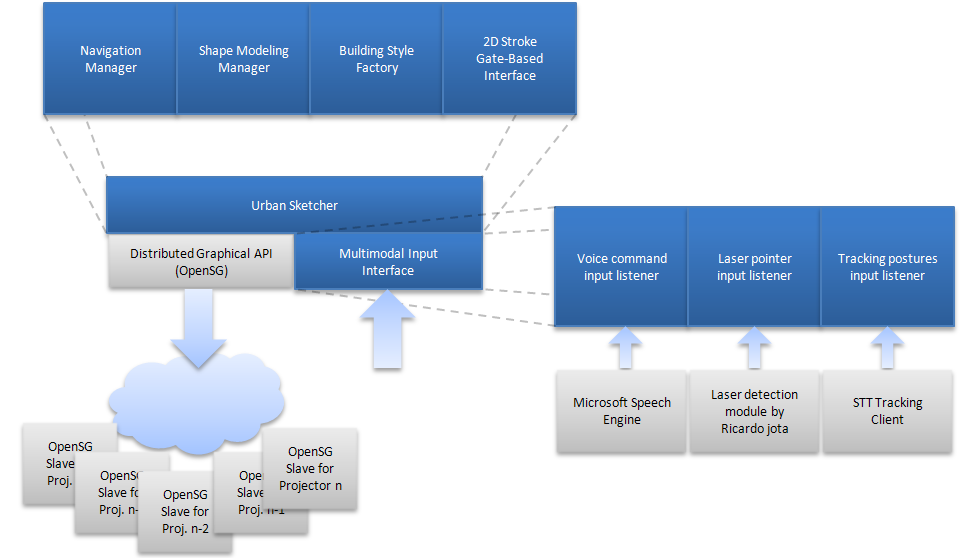
\includegraphics[width=16cm]{gfx/charts/block-diagram.png}
		\caption{Urban Sketcher Architecture Diagram}
		\label{fig:block-diagram}
\end{figure}

%\TODO{REMOVE 'ricardo jota'; add mouse input; add broadcast and remove input arrow}

Urban Sketcher is made of the following items\footnote{Blue items denote work done by the author.}:

The \textbf{Navigation Manager} is
		responsible for assembling navigation data from
		both voice and tracking input, along with gate events which trigger navigation changes,
		supporting several navigation modes;
	
The \textbf{Shape Modeling Manager} is
		responsible for representing a 3D editable shapes
		along with their geometry information and supporting a range of operations;
	
The \textbf{Building Style Factory} is
		responsible for parsing building style definitions
		and converting blueprints and building height into actual building instances;
	
The \textbf{2D Stroke-Based Interface} is 
		a set of interface widgets and their controllers,
		supporting option gates, ring menus and stroke-based operation handling.
Urban Sketcher gets input from several media:
laser pointers, the server machine's mouse and optionally voice commands and tracking postures.
The system can render real-time views to any number of slave machines.
An XML configuration allows parameterizing the range of affected machines and topology of the rendering slaves,
so rendering solely on the server, to a large screen display or both is a matter of switching configurations.


\section{Stroke-Based Input Interface}

This section details the concepts used in the creation of the interface for the system.

\subsection{Strokes}

A stroke is the result of continuous input from one laser pointer, from the time the laser
light button is pressed until it is released. 

By using the laser detection module, the system gets a stream of laser readings which
come sequentially tagged, that is, the module identifies with reasonable success when different strokes
occur simultaneously, returning both readings tagged with different stroke IDs.
Even so, the module can't infer whether different strokes came from the same source laser pointer.

This limitation sets an important assumption in our system -- one can not know whether 2 strokes came
from the same user, therefore operations must take place during at most the stroke period.

Strokes can also be emulated by using a mouse and pressing
the button as if it were a laser pointer.


\subsection{Gates}

The most common activation action in current Graphical User Interface (GUI) computer interactions works
by displaying a button on the screen and the user activating it by pressing the pointer device's button.
Given that users will rely on laser pointers to interact with the system's GUI, a limitation derives from
using them instead of mice or track balls -- while a user isn't pressing the laser light button,
neither the system nor the user can accurately know where on the screen the laser is pointing to.
In order for the user to see the laser projection on the screen he must be pressing the button.
This system requires a different GUI solution.

Based on prior research by \cite{CROSSY}, the gate concept was implemented with slight changes.

A gate is an imaginary two dimensional line on the screen, bound by two visible extremes.
In order to activate it, one must draw a stroke which crosses the imaginary line, effectively crossing the gate
(see Fig.\ref{fig:activation}).

Gates can feature a text label or a suggestive image to symbolize the action they perform.
It was decided not to mix both representations -- if the gate is illustrated, a tooltip can be invoked
by approaching the gate's area of influence without crossing it, so the tooltip can be read and the action optionally avoided.

\begin{figure}[ht]
	\centering
		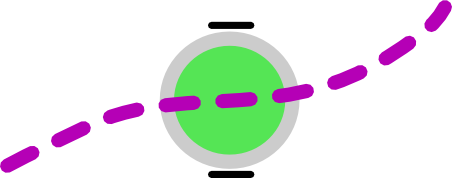
\includegraphics{gfx/activation.png}
		\caption{Gate activation}
	\label{fig:activation}
\end{figure}



\subsection{Menus}

\TODO{REVIEW TEXT...}
The menus of this system are ring-shaped, with the options (gates) spread along the ring.
The menu's background ring is translucent so the main viewport remains visible and each background color
depends on the functionality it offers.
On the bottom-right area a curved label identifies the menu title.
The top-right area features additional gates for the dismissal of the menu, moving it around and
returning to the main menu if at a subsequent level (see Fig.\ref{fig:menu}).

A lot of effort has been put for menus to be usable. On cases where menus offered a large number of actions/options,
those were clustered into modes to keep a conveniently small number of visible options.
On such menus, a set of gates at the left side of the menu represent the available modes.
Selecting a different mode is a matter of activating the respective illustrative gate.

%Submenus are another way of clustering options. \TODO{...}


\begin{figure}[ht]
	\centering
		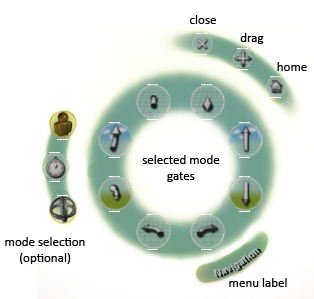
\includegraphics[scale=0.75]{gfx/menu.png}
	\caption{Menu and its areas}
	\label{fig:menu}
\end{figure}




\subsection{Stroke Gestures}

To invoke the main menu the user needs to draw a closed stroke resembling a triangle (see Fig.\ref{fig:triangle}).
When such stroke is drawn one main menu instance appears centered on it.

\begin{figure}[ht]
	\centering
		
\includegraphics[scale=0.75]{gfx/triangle.png}
	\caption{Main menu stroke}
	\label{fig:triangle}
\end{figure}


Besides menus derived from the main menu tree, which is invoked as we've just seen by drawing a closed triangle stroke,
there are menus which focus on an existing shape on the 3D world.
These are called contextual menus and they can be invoked by selecting a desired shape's face or edge.
To select a face one has to draw a small stroke starting and ending inside the face.
To select an edge one has to draw a small stroke starting on one of the edge's neighboring faces and ending at the remaining one,
effectively crossing the edge to select it (see Fig.\ref{fig:face-edge-selection}).


\begin{figure}[ht]
	\centering
		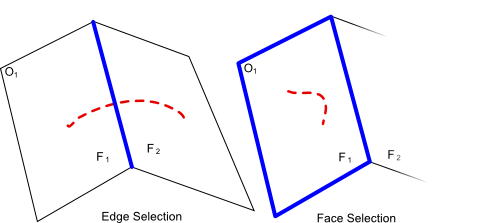
\includegraphics[scale=0.75]{gfx/face-edge-selection.png}
		\caption{Edge and Face selection}
	\label{fig:face-edge-selection}
\end{figure}



\section{Multimodal Input Interface}

Using laser input allows the usage of all system's functionalities.
Even so, an alternative arm-tracking and speech recognition command interface exists to enhance particular tasks.
The arms are tracked by attaching 2 reflective markers on each arm: one on each wrist and one close to each elbow.
Speech commands are obtained from a wireless headset attached to the user's ear (see Fig.\ref{fig:markers2}).


\begin{figure}[ht]
	\centering
		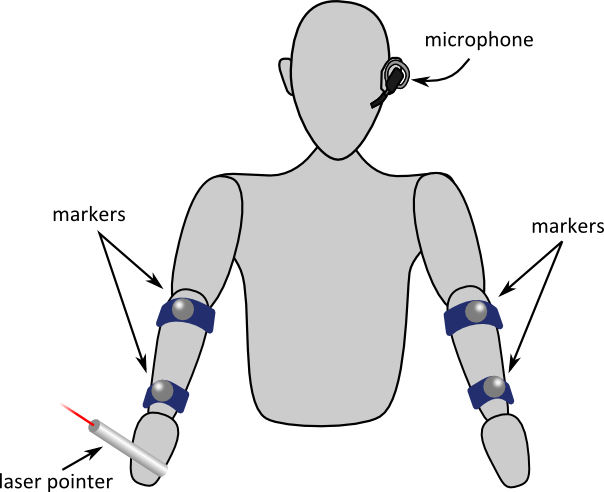
\includegraphics[scale=1.3]{gfx/markers2.png}
	\caption{user with reflective markers and wireless headset}
	\label{fig:markers2}
\end{figure}



\subsection{Arm Posing Flight Mode}

The flight mode is an alternative navigation mode. Since it affects the point of view, this task can't be performed by
several people simultaneously, therefore unlike most of the system this navigation mode has global states
-- the user might be either stationary of flying (see Fig.\ref{fig:flight}).

The user starts interacting by having his arms extended toward the screen.
In order to begin flying the command ``Begin flying'' must be given.
To stop at any time one only needs to say ``Stop flying''
\footnote{Although semantically inconsistent, the words begin and stop were used after performing speech recognition
tests with both start/stop, begin/end and begin/stop, concluding that this combination had the better recognition ratio.}.

Controlling flight speed works by measuring the distance between hands -- the closer they are to each other the faster
the flight speed is. If the arms do a wide enough angle between them the flight comes to an halt.
Changing the flight orientation relatively to the ground is achieved by setting the arms angle with the ground at opposing directions,
with a bigger difference between these angles generating a faster rotation movement. If the user wants to turn right, for instance,
he has to raise the left arm and lower the right one.

To change flight altitude both arms must be oriented in the same direction relatively to the ground plane
-- either both raised or lowered. Again, the higher the angle is from the original forward pose position
the bigger the flight altitude shift is.

\begin{figure}[ht]
	\centering
		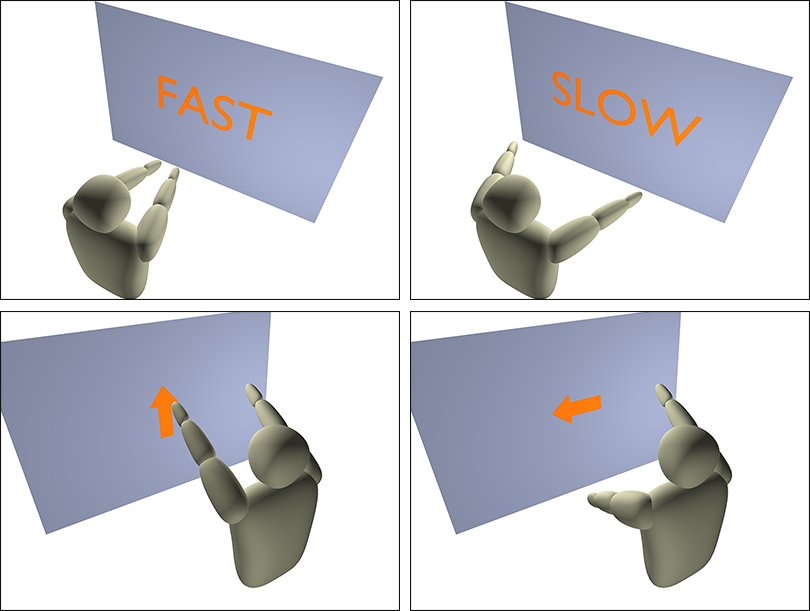
\includegraphics[scale=0.3]{gfx/flight.png}
	\caption{Flight mode: controlling speed and direction}
	\label{fig:flight}
\end{figure}



\section{Content Creation Concepts}

\subsection{Apply-to-Scene Creation}
\label{design:apply-to-scene}

To create a new object on the scene one has to perform a stroke which activates the desired shape creation gate (cube for instance)
and continue the stroke onto the desired location where the shape is to rest. As soon as the gate is activated the shape appears
on top of the stroke and keeps following the stroke until it ends, offering a preview of the location where is would rest
if the stroke ended that particular moment (see Fig.\ref{fig:apply-to-scene}).
To figure out the actual location for the shape during the task the shape is iteratively collided against the
existing scene geometry so it stays in touch with the environment.

\begin{figure}[ht]
	\centering
		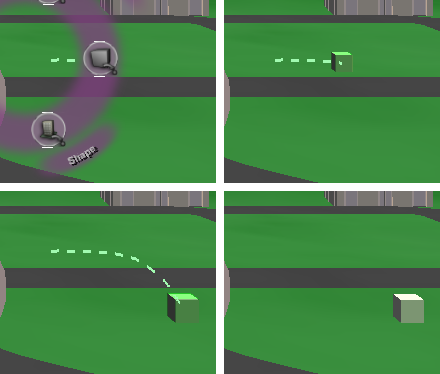
\includegraphics[scale=0.5]{gfx/apply-to-scene.png}
	\caption{Apply-to-scene procedure - creating a shape}
	\label{fig:apply-to-scene}
\end{figure}



\subsection{Instancing a Building}
\label{design:building}

To create a building one has to feed the system 3 parameters: building style, blueprint and height.
Due to the system decision for stroke-driven actions without global state, these 3 parameters are given with the
minimum strokes (2), as described next.
From a menu the list of supported building styles is presented to the user, each style a different gate.
Once activating the desired style the user starts an apply-to-scene process, moving a construction plane which must
be put where the blueprint is to be drawn.
The user draws a closed rectangle representing the blueprint and after closing it continues
the stroke upwards in order to define the building's height.
Once the stroke ends the building is generated according to the given parameters.
The construction plane has now carried out its purpose and therefore is terminated (see Fig.\ref{fig:building}).

\begin{figure}[ht]
	\centering
		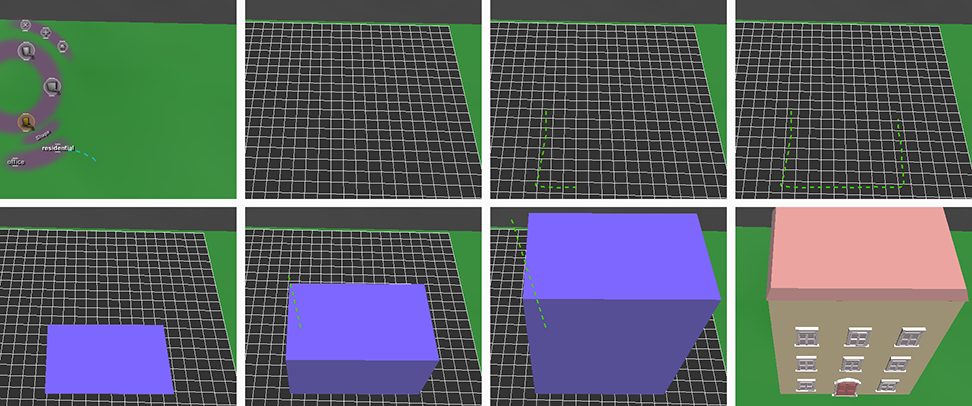
\includegraphics[scale=0.4]{gfx/building.png}
	\caption{Building creation procedure}
	\label{fig:building}
\end{figure}


\chapter{Implementation}
\chapter{Implementation}

\TODO{intro to implementation}


\TODO{IMMIVIEW OVERVIEW?}
%\section{ImmiView Framework}

\subsection{Architecture}


\section{General Interface}

\subsection{Strokes}

A \emph{stroke} is a continuous set of points drawn on our system.
Since the system works both on Tablet PCs and on power walls,
a stroke can be drawn either with the tablet's pen or with
a regular laser pointer.

Drawing strokes is therefore the main way of users interaction with
the system. It has been built to support several users interacting
simultaneously in the screen.

With this approach, any component in the system can't make use
of global mode information due to the fact that one can't know
for sure if the $ stroke_{n+1} $ was drawn by the same user than $ stroke_{n} $.

Therefore, strokes must serve many purposes, and in cases where a sequence
of actions must be done in order, they're achieved under the same stroke.

Another decision taken early on in the implementation was that there shall not be
fixed areas in the screen for contents such as menus. The initial state of the
system is completely free of interface widgets. When starting the system the users
see only a 3D perspective of the virtual world.


\subsubsection{Stroke Actions}

Any stroke can be interpreted as being one of (see figure \ref{fig:lasso-tri}):

\begin{description}
		\item[an open stroke] --
				any stroke where the segments don't intercept each other;

		\item[a lasso] --
				a closed stroke;

		\item[a triangle stroke] --
				this is a special case of a lasso, i.e. closed, where the stroke resembles a triangle.
\end{description}


\begin{figure}[!ht]
		\centering
		
\includegraphics[width=3.5cm]{gfx/lasso.png}
		\qquad\qquad\qquad
		
\includegraphics[width=3cm]{gfx/triangle.png}
		\caption{Lasso and triangle strokes}
		\label{fig:lasso-tri}
\end{figure}


\subsection{Gates}

As described earlier on in section \ref{sec:gate-concept} The Gate Concept,
a gate solves the problem of our input devices not being capable of detecting
click actions consistently.

\begin{figure}[!ht]
		\centering
		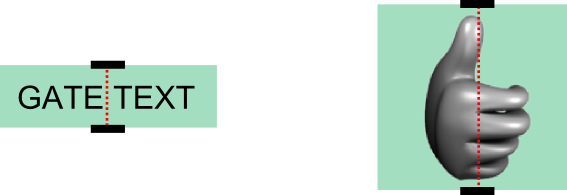
\includegraphics[width=5cm]{gfx/gate1e.png}
		\vspace{-0.5cm}
		\caption{Two gates: one featuring text and the other visual content}
		\label{fig:gate1}
\end{figure}

\begin{figure}[!ht]
		\vspace{-0.7cm}
		\centering
		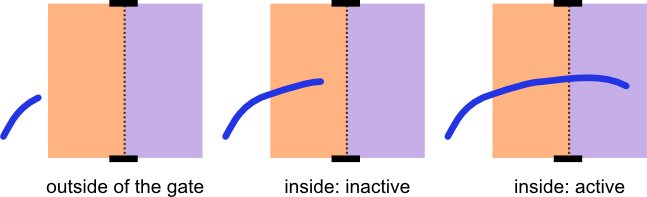
\includegraphics[width=10cm]{gfx/gate2e.png}
		\vspace{-0.5cm}
		\caption{Gate activation}
		\label{fig:gate2}
\end{figure}

\begin{figure}[!ht]
		\vspace{-0.7cm}
		\centering
		
\includegraphics[width=3cm]{gfx/gate3e.png}
		\vspace{-0.5cm}
		\caption{Gate showing its tooltip}
		\label{fig:gate3}
\end{figure}


Gates can either have text our visual content (fig \ref{fig:gate1}).
It was decided that gates shouldn't feature both at the same time.

The activation takes place by entering both the left side and the right
side areas of the gate consecutively (or the other way around).
The dashed line in figure \ref{fig:gate2} is only imaginary.

In order for users to inspect the meaning a gate with visual content, a
tooltip appears when the stroke is inside the gate,
which will happen prior to activation, so users can give it up (figure \ref{fig:gate3}).

In conclusion, for a user to activate a gate, an horizontal or quasi-horizontal
stroke must be drawn, as seen in figure \ref{fig:gate4}.

\begin{figure}[!ht]
		\centering
		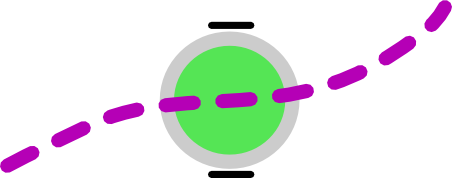
\includegraphics[width=4cm]{gfx/activation.png}
		\caption{gate activation example}
		\label{fig:gate4}
\end{figure}

\subsection{Menus}

In order to get the main menu, the user has to draw a closed triangle stroke.
The menu appears at the center of the drawn stroke.

\begin{figure}[!ht]
		\centering
		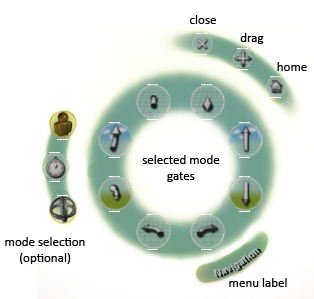
\includegraphics[width=8cm]{gfx/menu.png}
		\caption{menu and its components}
		\label{fig:menu}
\end{figure}

Menus are round and have additional auxiliary gates and labels (figure \ref{fig:menu}).

In the bottom right area a label clearly identifies the functionality provided by the menu.

In the top right area menus feature a set of special gates.
The \emph{close gate} dismisses the menu.
The \emph{move gate}, when activated, makes the menu follow the stroke position until it ends.
The \emph{home gate} allows the user to go back to the previous menu, when that action applies.

Occasionally the menus are too complex and need to be segmented.
When that happens, mode selection gates appear to the left of the menu.

Different menus have different background colors.
They're translucent so the main perspective remains partially visible.
Menu colors were chosen to reflect the functionality, ex: all navigation menus are green.



\section{Navigation}

\subsection{1st Person Navigation Mode}

\TODO{ADD 1ST PERSON SHOT}
This widget has four moving directions and four rotations.
It allows to move forward/backward,
go up/down,
turn left/right and
pitch up/down.

Crossing a gate once starts the movement.
Crossing it again stops it.
If a gate is crossed while another one is active,
the first one stops -- this behavior was enforced
by user test inspection.
Having several moving/rotation
actions applied at the same this is confusing.
Clarity was favored over efficiency.

\subsection{Compass Navigation Mode}

\TODO{ADD COMPASS SHOT}

This is a direct application of the concept defined
in section \ref{sec:bev} Bird's Eye View Mode, on page \pageref{sec:bev}.

The outer ring of the widget allows the user to see and change
the current orientation in terms of cardial points positioning.

The inner circle allows inspection of the top-down view, with the user
being in the center. Applying strokes inside this area drags the map,
changing user's position in the ground plane.

\subsection{Examine Navigation Mode}

\TODO{ADD EXAMINE SHOT}

\TODO{ADD VIRTUAL SPHERE ILLUSTRATION}

This widget features a wire frame sphere at the center, two zooming gates
and two additional gates whole purpose is described below.
It is a direct application of the concept defined
in section \ref{sec:examine} Examine Navigation Mode, on page \pageref{sec:examine}.

The sphere occupying the center of the widget simulates the virtual sphere centered
on the subject of interest with radius $ dist $.

The user is at distance $ dist $ from the subject of interest.
This distance can be increased or decreased by activating the zoom gates.
Movements in the $ XX $ direction are translated into rotations around $ \theta $, while
movements in the $ YY $ direction translate into rotations around $ \phi $.

Two additional gates allow changing the subject of interest.
They work by crossing and ending the stroke at the target.
The first one, \emph{point of interest center}, allows one to examine the center of the object.
The remaining one, \emph{point of interest spot}, changes the examined position to be the surface
position where the stroke ``touches''.
The former is useful for inspection of the overall object while the latter is of great
use in editing or inspecting surface details.

\subsection{Fly Navigation Mode}

%intro DONE

\begin{figure}[!ht]
		\centering
		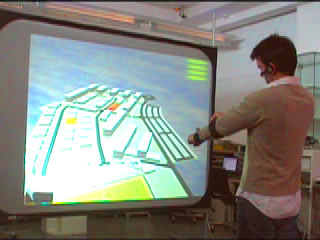
\includegraphics[width=6cm]{gfx/don.png}
		\caption{user navigating with the multimodal navigation mode}
		\label{fig:don}
\end{figure}

Navigation in a 3D scene takes place normally using a desktop computer
with the mouse and keyboard as input devices and the monitor as output device.
In the multimedia lab there was a motion tracking system available.
It was put to use in conjunction with a wireless microphone to allow for an
alternative mode of navigation. A set of reflective markers is attached to
the user's arms and the wireless microphone attached to his/her ear.
The microphone allows for enabling and disabling the multimodal navigation mode
by issuing respectively the commands \textbf{begin flying} / \textbf{stop flying}.

\subsubsection{Physical Configuration}

Motion tracking took place using reflective markers attached to the user's arms (figure \ref{fig:markers-cams} left).
A set of 4 cameras with infrared lights were installed in the lab, which each
captured image being processed by a computer identifying the visible markers in
image-space, making the computation of the spacial position of each marker by
merging the data from the 4 captured views and labeling each tracked marker
from the initial extended arm pose (figure \ref{fig:markers-cams} right).

The Microsoft Speech API 5.1, American English version was used to recognize the
voice commands. Capturing of the commands was done by attaching a wireless microphone
to the user's ear.

%ap�s a compara��o do reconhecimento do mesmo face a um microfone fixo e um Bluetooth.

%O reconhecedor mostrou-se algo limitado, tendo sido necess�rio adaptar a gram�tica a palavras n�o amb�guas entre si ou
%que gerassem falsos positivos.
%
%%Preliminarmente realizou-se um teste para escolher o melhor hardware para reconhecimento de voz, entre um microfone Wireless, %um fixo a captar toda a sala e um auricular Bluetooth. Os comandos dispon�veis na aplica��o foram ditados repetidas vezes por 3 %utilizadores, em ordem aleat�ria e com os 3 dispositivos.
%
%%Conclui-se que o microfone Wireless era a melhor op��o com uma taxa de reconhecimento m�dia de 99\%, mas para dist�ncias curtas %(\(<\)3m) o auricular Bluetooth teve resultados semelhantes, com 98\%. O microfone fixo captou muito ru�do e produziu resultados %muito insatisfat�rios de menos de 50\%.

%O reconhecedor mostrou-se algo limitado, tendo sido necess�rio adaptar a gram�tica a palavras n�o amb�guas entre si ou
%que gerassem falsos positivos.

\begin{figure}[!ht]
		\centering
		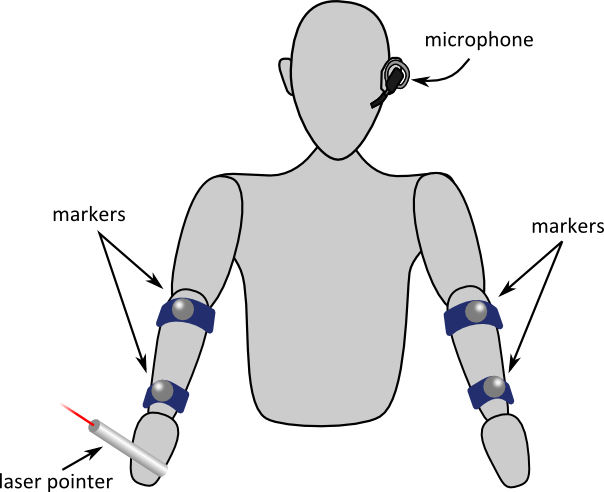
\includegraphics[width=7cm]{gfx/markers2.png}
		\qquad
		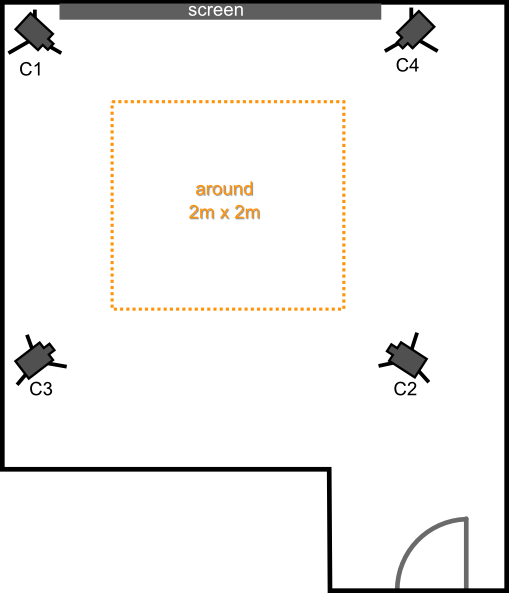
\includegraphics[width=5cm]{gfx/4cam-setup.png}
		\caption{markers and camera setup}
		\label{fig:markers-cams}
\end{figure}
%
%
%\begin{figure}[!ht]
%		\centering
%		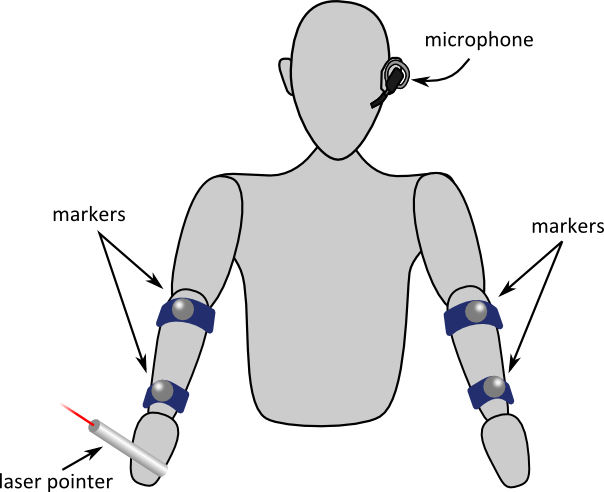
\includegraphics[width=6cm]{gfx/markers2.png}
%		\caption{markers and microphone for tracked user}
%		\label{fig:markers}
%\end{figure}
%
%\begin{figure}[!ht]
%		\centering
%		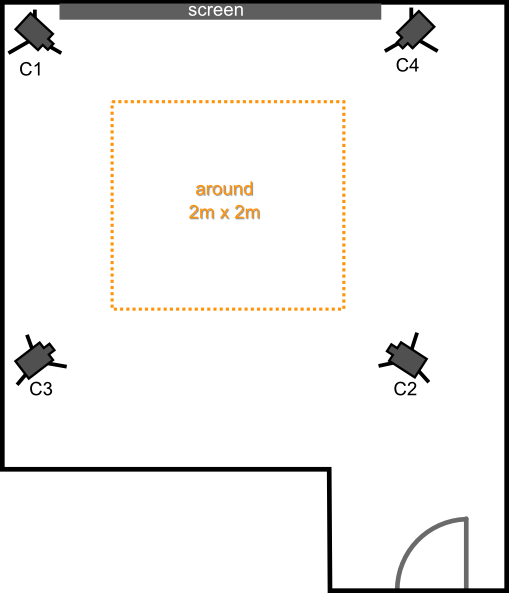
\includegraphics[width=6cm]{gfx/4cam-setup.png}
%		\caption{four cameras setup for motion tracking}
%		\label{fig:cam-setup}
%\end{figure}


\subsubsection{Interaction}

The multimodal navigation mode requires the user to have his / her arms extended towards the screen.

Controlling the flight speed works by the measurement of the distance between hands:
the closer they are from each other, the faster the flight speed is.
If the arms get close to a ninety degrees angle between them the flight halts (figure \ref{fig:fly-speed}).

Changing the flight orientation relatively to the ground plane is achieved by setting the arms
angle with the ground at opposing directions, with a bigger difference between angles generating
a faster rotation movement. If the user wants to turn right, for instance, he / she has to
raise the left arm and lower the right one (figure \ref{fig:fly-rot-up}, left).

To change flight altitude, both arms must be oriented in the same direction relatively to the ground plane,
either both raised or both lowered.
Again, the higher the angle is from the original arms extended forward pose,
the bigger the flight altitude shift occurs (figure \ref{fig:fly-rot-up}, right).

\begin{figure}[!ht]
		\centering
		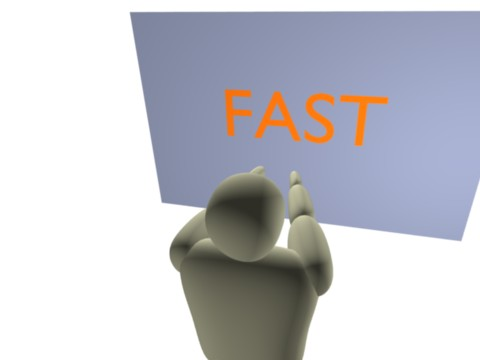
\includegraphics[width=5cm]{gfx/immi-fly-fast.jpg}
		\qquad
		
\includegraphics[width=5cm]{gfx/immi-fly-slow.jpg}
		\caption{control flight speed}
		\label{fig:fly-speed}
\end{figure}

\begin{figure}[!ht]
		\centering
		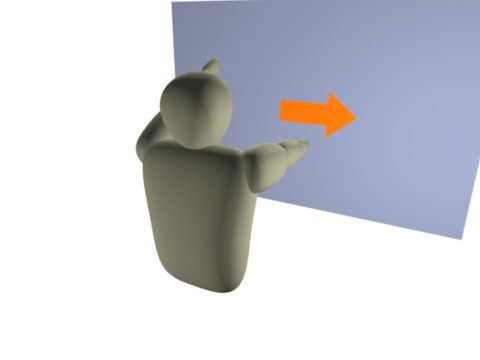
\includegraphics[width=5cm]{gfx/immi-fly-rotate.jpg}
		\qquad
		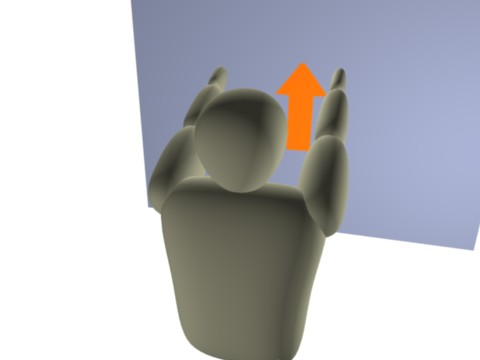
\includegraphics[width=5cm]{gfx/immi-fly-up.jpg}
		\caption{rotate flight orientation and increasing flight altitude}
		\label{fig:fly-rot-up}
\end{figure}

%
%\TODO{IMMI PAPER}



\section{Building Creation}

\section{Custom Shape Creation}

\TODO{CV PAPER}



\section{Custom Shape Creation}

The purpose of this functionality is to grant the user a simple yet robust shape
structure supporting a set of geometry transformation operations,
so that custom shapes can be modeled with ease. Figure \ref{fig:example} shows an example result.

\begin{figure}[!ht]
	\centering
	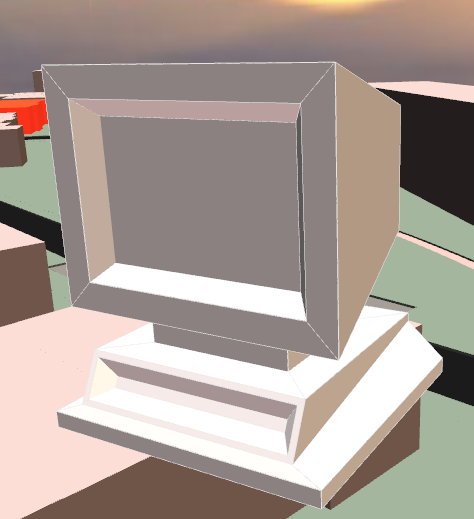
\includegraphics[width=5cm]{gfx/ex-monitor.png}
	\caption{monitor shape modeled in the system}
	\label{fig:example}
\end{figure}

\subsection{Internal Structure}

The defined structure to support the custom shape is based on 4 sided faces.
This decision implies that:
\begin{itemize}
	\item every edge is shared by two faces;
	\item every edge in a face has an opposite edge relating to that face.
\end{itemize}

Besides the \emph{list of vertices} and its positions and the \emph{list of faces}
(each face being a list of 4 vertex indices),
an additional structure is computed: the \emph{edge map}.
It maps which faces share each edge.
This information is used to optimize the low-level operations for
getting the opposite edge and getting the face loop,
a	paramount to the split face loop operation.

Aside from these data structures which hold the shape's form,
there's a \emph{list of face colors}, one per face, to hold the shape's appearance.

These shapes support the undo operation. It was implemented based on the Memento design pattern \cite{despat}.
Each object has an associated stack of states, so the user can return to any previous state of modeling if needed.


\subsubsection{Persistence}
\label{sec:shape-persistence}

Each modeled object is responsible for saving its geometry data.
The chosen format for persistence was XML and each shape is translated into an XML element.

The format resembles the simplified structure of a WaveFront OBJ file, but described in XML.
The vertices are listed, starting from index 0.
Next each face is defined as an ordered list of 4 vertex indices.
The list of colors, one for each of the faces, is described in the end.

\begin{small}
	\begin{verbatim}
	<?xml version="1.0" encoding="utf-8"?>
	  <shape>
	    <vertices count="56">
	      <vertex x="-1" y="-0.627882" z="5.29942"/>
	      ...
	    </vertices>
	  <faces count="54">
	    <face v1="0" v2="1" v3="2" v4="3"/>
	    ...
	  </faces>
	  <colors count="54">
	    <color r="0.9" g="0.9" b="0.9"/>
	    ...
	  </colors>
	</shape>
	\end{verbatim}
\end{small}

\TODOL{CLASS HIERARCHY, PROVIDED SHAPES (from CV document)}

\subsubsection{Relevant Algorithms}

\paragraph{Bevel Face}

\begin{figure}[!ht]
    \centering
    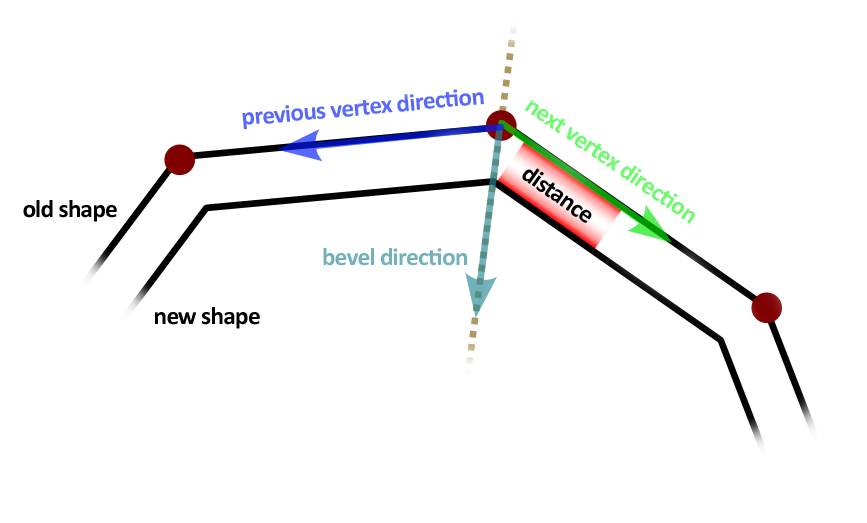
\includegraphics[width=9cm]{gfx/bevel.png}
    \vspace{-1cm}
    \caption{Main directions and relations supporting the bevel operation}
    \label{FIG-GS-BEVEL}
\end{figure}

The algorithm used for beveling faces uses, for each vertex,
the directions from it to the previous and next vertices,
averages it and normalizes it, getting the bevel direction vector with unit length.
The new vertex position is then:

\begin{equation}
	v^{'} = v + b_{dir} \cdot b_{distance}
\end{equation}


\paragraph{Determining Edge Directions}

\begin{figure}[!ht]
    \centering
    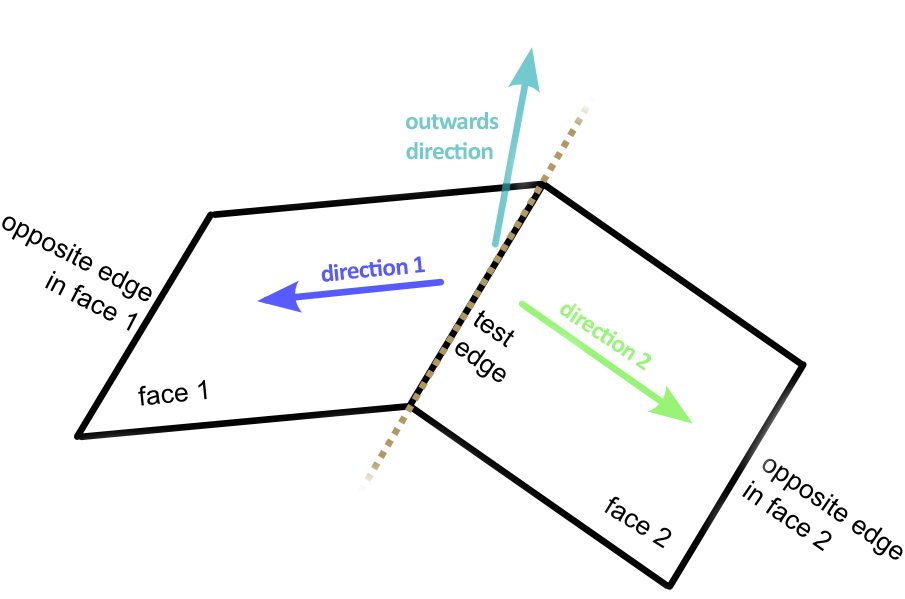
\includegraphics[width=9cm]{gfx/face-dirs.png}
    \vspace{-0.5cm}
    \caption{Determining edge directions from neighboring faces}
    \label{FIG-GS-FACE-DIRS}
\end{figure}

The most relevant directions according to an edge are those along the faces
which share it and the direction farthest away from the other ones.
 
Calculating direction 1 is easy once the edge map is calculated
and getOppositeEdge(edge) function defined.

Direction 2 works the same way, this time following the remaining direction.

The outwards direction resembles the concept of a face normal but applied to an edge
-- it points out relating to the neighboring faces.
This direction can be easily found by averaging the face normals
for the faces containing the selected edge.


\subsection{User Interface}

\emph{Face selection} occurs by drawing a stroke exclusively over a face.

\emph{Edge selection} occurs by crossing the desired edge, with the stroke beginning
on one of its neighboring faces and ending on the remaining one.
Figure \ref{fig:selection} illustrates this procedure.

\begin{figure}[!ht]
	\centering
	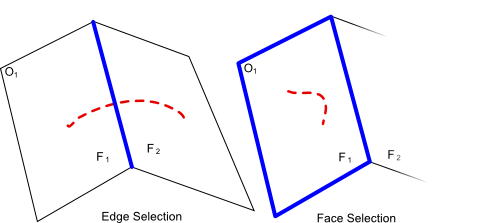
\includegraphics[width=11cm]{gfx/face-edge-selection.png}
	\caption{edge and face selection}
	\label{fig:selection}
\end{figure}

Once the component gets selected, a contextual menu appears in the vicinity
of the selection, allowing the user to select the operation to apply (see figure \ref{fig:contextual}).

\begin{figure}[!ht]
	\centering
	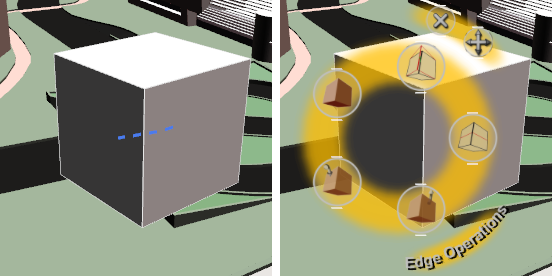
\includegraphics[width=10cm]{gfx/contextual.png}
	\caption{activation of a contextual menu from an edge selection}
	\label{fig:contextual}
\end{figure}

In several of the supported operations one of the parameters is direction.
In those cases the nearest vector direction algorithm is used.
The direction of the ongoing stroke is compared with the set of suggested directions,
with the closest direction being applied in real-time, a mechanism commonly
named \textit{snapping} (see figure \ref{fig:election}).

\begin{figure}[!ht]
	\centering
	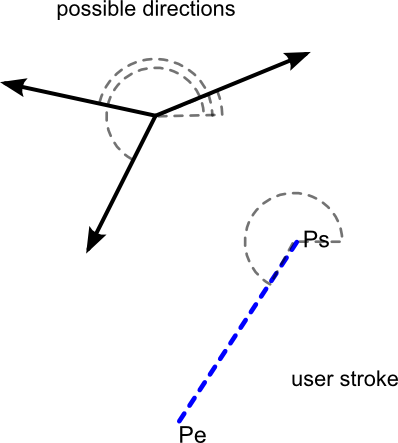
\includegraphics[width=5cm]{gfx/election.png}
	\caption{electing the nearest vector direction}
	\label{fig:election}
\end{figure}

\subsection{Supported Operations}

A description of the supported operations and their provided directions for modification follows,
as seen in figure \ref{fig:shots}.

\begin{figure}[!ht]
	\centering
	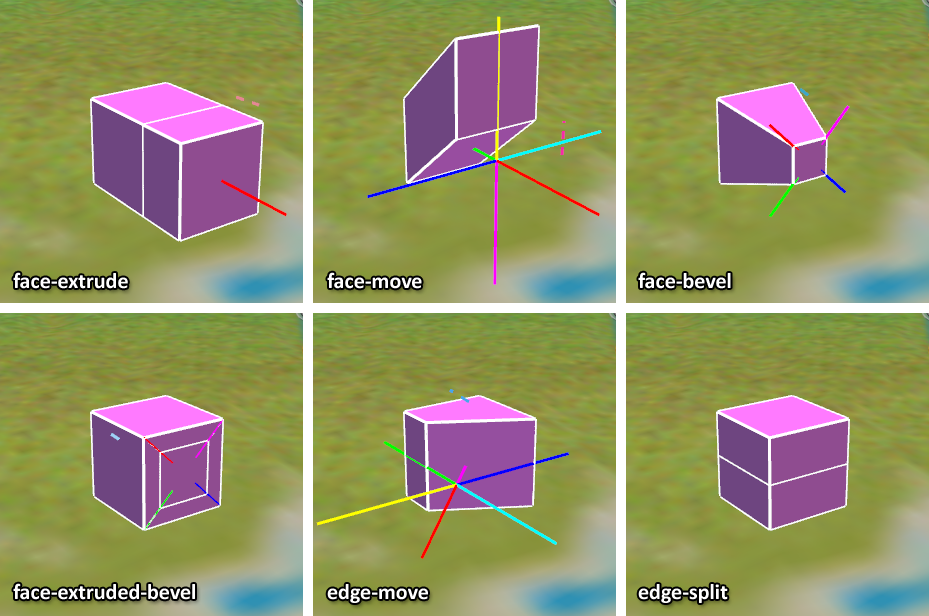
\includegraphics[width=11cm]{gfx/gs-ops.png}
	\caption{geometry manipulation operations}
	\label{fig:shots}
\end{figure}

\subsubsection{Geometry Manipulation Operations}

\begin{description}
	\item[Face Extrude] --
		the direction is extracted from the selected face normal. Displacement based on stroke length.
		
	\item[Face Bevel] --
		the bevel distance depends on the stroke length.
		
	\item[Face Move] --
		this operation supports not only the face normal directions,
		but also the directions from the face center towards the four boundary edges.
		
	\item[Edge Move] --
		supports the edge normal along with the directions from it towards its neighboring faces.
		
	\item[Edge Split] --
		this operation occurs immediately since it doesn't require any real-time input from the user.
		The sketched cut propagates throughout the intrinsic selected face loop, each edge cutting
		the opposite edge in each face of the loop, until either no more faces occur or an already
		visited face is revisited. \TODOL{FIGURE FOR THIS PROCEDURE?}
\end{description}

\subsubsection{Other Operations}

\begin{description}
	\item[Undo] --
		any shape operation previously defined can be reverted.
		
	\item[Loading and Saving] --
		the object can be loaded from or saved to the XML format defined above.
		Exporting content from an external 3D modeler is straightforward.
		An exporting plug-in for Blender was implemented in Python.
\end{description}




\section{Custom Scenery Creation Work Flow}

\TODO{blender, XML...}

\TODO{summary of implementation}




\chapter{Evaluation}
\label{cha:evaluation}
\TODO{intro to evaluation}

\TODO{Scenarios}

\TODO{modeling capabilities of geosculpt against blender or sketchup (both in time and expressivity)}

\TODO{tests made for improve}

\TODO{last test}

\TODO{summary of evaluation}


\chapter{Conclusion}
\chapter{Conclusion}

\TODO{intro to conclusion?!}

%%%%%%%%%%%%%%%%%%%

% motivation

The produced work was made to provide architects a way
of exploring large scale displays for the creation of urban sceneries.
This task can be performed collaboratively using common laser pointers.
The implementation of a set of navigational modes allow for easy
exploration of complex 3D scenes.
This scenario allows showcasing and reviewing of projects with clients.

The support for tablet PCs permits a portable and cost-effective alternative
to the large display screen.

A building creation method was developed that provides a fast way
of generating buildings based on their facade blueprints and height and
setting its purpose, with the system generating walls and facades that
reflect the choices made.


% aplicabilidade

\section{Main Contributions}

% work flow
This system was thought out to aid the task of generating 3D buildings.
An alternative work flow was defined where digital content supplied by
the municipal government or other entity is put to use -- a virtual 3D
version of the terrain is the starting point for the projection of
architectural buildings.
With it users have a way of generating buildings using a set of
architecture styles to generate its facades, wall materials and roof,
and they can do it surrounded by a simulation of the environment.

% u s concepts
For this task several concepts were introduced -- facade attachments,
template shapes, custom shapes and architecture styles.
Facade attachments can be generated from a 3D modeler such as Blender,
using an exporter plug-in to export the content into the internal shape format.
Architecture styles can also be created by users, providing a 
powerful way to define ``recipes'' for building creation, by setting the
odds of a certain type of door, window, balcony etc appearing in the facade,
setting floor height and layout, facade wall color and texture and roof type.

% custom shapes
In cases where custom 3D shapes are needed to fulfill a particular aspect
of a building, the user has the ability to create custom shapes.
These can be edited by a small set of face and edge operations,
studied to cover the most common needs of geometry modeling.
The most useful directions are available for the user to manipulate the
faces and edges, without the overhead of dozens of menu commands and parameters
so common in nowadays 3D modeling software.

% gates e menus
In order to solve the limitations of using laser pointers / tablet PC pens
for interaction, the gate concept was developed and exploited.
It provides a way of activating options by drawing strokes instead of clicking.
Stroke continuity data was used: the set of events from the start of the stroke
until its ending, passing through gates can trigger complex operations
such as dropping a shape from a menu into the 3D view.
A non-intrusive menu form was defined and applied, with a minimalistic approach
at the starting interface, letting the users invoke and position menus as they see fit.

% navigation modes
A set of navigational modes was developed to cover the most common exploration
and inspection tasks.
The common walk / fly mode was made available to give users the
possibility of exploring the scene as real users would. 
The compass navigation mode allows for seeing a top-down view of the nearby map,
allowing dragging the map for movement and  rotating the orientation
via a ring showing the cardinal points.
The examine navigation mode provides an effective way of inspecting an object of any
scale by dollying around it. The examined object or surface can be easily changed.
Having a motion tracking system installed, one can also fly using the arms.
This has proven both pleasing and effective, empowering the user of an alternative
way to rotate, change the altitude and flight speed by making use of arm movements.

%%%%%%%%%%%%%%%%%%%

\section{Future Work}

There is space for improvement in several aspects of the project,
even more since it addresses so many areas.

% work flow
The integration of real terrain data into the system could be eased by
the direct support of height maps, topography maps data such as contour lines
and aerial photographies. A work flow for the importing of such content is
even so outlined.

The facade walls could have forms other than rectangles and most work was
done so that such change could be easily supported, as long as a good
interface is provided to input such blueprints.

% realism
Lighting conditions could be manipulated inside the program with an
accurate simulation of daylight and shadowing, a subject highly valued
by architects for the definition of the location where a building is to be built.

Textures and materials could make usage of the latest developments in GPU
technology to simulate metals, glass and other materials and
techniques such as bump maps to give greater depth to facade details and textures.

% modeling operations
A more elaborate set of operations could be supported for modeling custom shapes.
Most operations could be generalized for application to a group of edges or faces.
Even so, the available operations are a good compromise between the complexity
of professional modelers and the stroke-based, minimalistic interface provided.

% voice
%Voice operations could 


%%%%%%%%%%%%%%%%%%%

\cleardoublepage
\bibliographystyle{alpha}
\addcontentsline{toc}{chapter}{\bibname} %\refname
\bibliography{dissertation}

%%%%%%%%%%%%%%%%%%%

%\part{\appendixname}
%\appendix

%\chapter{Appendix One}
%\label{cha:appendix-1}
%\section{Section One}

xxx

%%%%%%%%%%%%%%%%%%%

%%%%%%%%%%%%%%%%%%%

\end{document}
